% Copyright (C) 2015 Chen-Pang He <http://jdh8.org/>
%
% This file may be distributed and/or modified under
%
% 1. LaTeX Project Public License
% 2. GNU Public License
%
% See the files COPYING.* for more details.

\documentclass{Amo}

\begin{document}
\title{矩陣運算}
\maketitle

\section{資料結構}
\begin{frame}{演算法 + 資料結構 = 程式}
    \begin{figure}
        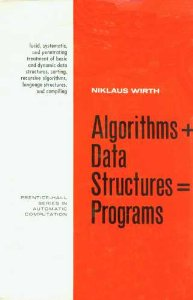
\includegraphics[height=0.5\textheight]{MatrixComputations/Algorithms_+_Data_Structures.jpg}
        \caption{Niklaus Wirth (1976).  \textit{Algorithms + Data Structures = Programs}}
    \end{figure}
\end{frame}

\begin{frame}{矩陣的儲存方向}
    \[ A = \begin{bmatrix}
        8 & 2 & 2 & 9 \\
        9 & 1 & 4 & 4 \\
        3 & 5 & 4 & 5
    \end{bmatrix} \]

    \begin{description}
        \item[橫向儲存] 8 2 2 9 9 1 4 4 3 5 4 5
        \item[縱向儲存] 8 9 3 2 1 5 2 4 4 9 4 5 
    \end{description}
\end{frame}
\end{document}
